\chapter{State of the Art}\label{chap:state-of-the-art}

This chapter describes the paradigms and characteristics of different programming languages. Thus concepts of compiled languages, interpreters optimizations and parallelism are discussed with respect of the different programming languages.


The purpose is to provide background information necessary to understand the study and present a clear justification for the decisions made


\section{Energy Efficient Systems}

An energy efficient system is defined as a system designed and optimized to performs its functions while consuming the minimum amount of energy possible, without compromising its performance, safety and reliability.

As \textcite{Muralidhar2020Energy} put it, the average power a system draws is:
$$P_{avg} = P_{dynamic} + P_{leakage}$$
The dynamic power depends on the $V$ supply, the clock frequency, the node capacitance and the switching activity. This power can be reduced by reducing the load on the chip or by manually setting a limit on how much voltage the chip can draw (known as undervoting \cite{undervolting-effects})


\section{System Architectures}

While the energy efficiency of a system is significantly affected by connected devices (e.g., a graphics card or an \gls{ai-accelerator}), this study excludes any external devices and expansion cards. Therefore, the processor architecture is the primary factor determining energy consumption on the system.

\subsection{x86 Architecture}
The x86 architecture is the most widely adopted in the world of desktop and server computers, whose market share is almost entirely shared by \href{https://amd.com}{AMD} and \href{https://intel.com}{Intel} who created it in 1978. Originally called x86-16, due to the 16 bit word size, it debuted in the Intel 8086 a single core, a $3 \mu m$ node processor.

Nowadays, the technology has improved, the architecture is now called x86-64, a 64 bit extension, created by AMD, and releases the full specification in August 2000. From 2006 onward, the two companies have been developing multicore processors, adding further \gls{SIMD} Extensions such as AVX-512 \cite{intel-avx512}. Then came the integrated graphics and finally Power Efficiency Focus. 

Then, a new paradigm came, instead of having a homogeneous set of cores, cores focused on performance and efficiency were added to the same package, the hybrid architecture. This set of heterogeneous cores meant the scheduler had to be changed in the operating systems, to better allocate more demanding programs on high performing cores and lower important tasks, such as background jobs to the highly efficient cores. This technology was released by Intel on the 12th generation Intel Core processors, using Intel 7 (a $7 nm$ node). This approach was revolutionary for power efficiency as \textcite{big-little} state.


\subsection{\gls{ARM} Architecture}
The \gls{ARM} (Advanced RISC Machine) is the newest architecture that has reached the global scale. Developed in 1986, the goal of this new 32 bit architecture was the simplicity. As \textcite{arm:story} puts it, the energy efficient came later. This allowed the \gls{ARM} architecture to dominate on the mobile sector, specially on smartphones, which run on batteries.

The characteristics of this \gls{isa} are a reduced set of instructions (\gls{RISC}), which  allows processors to have fewer transistors than \gls{cisc} architectures such as x86, resulting in lower cost, lower temperatures and lower power consumption.

Currently, this technology is not only used in low-power light devices, but many laptops, and even desktops are using \gls{ARM} chips due to their power efficiency and performance \cite{arm:optimization-big.LITTLE}.

\gls{ARM} also has a hybrid technology, called big.LITTLE, as described by the \cite{arm:biglittle2013}{ \gls{ARM} White Paper} that combines high-efficiency cores and high-performance cores. This architecture dominates the mobile device market and is increasingly found in modern laptops. 




\subsection{CPU Design for Multi-core dies}
Is it important to note that a computer that reports having more than 32 logical cores, usually has more than one socket, thus the performance and scaling of programs on multiple sockets can affect the energy efficiency and performance. This is due to the fact that information has to move between the multiple cache levels. 

From \cite{phd-apmtrlk}'s Table 2.1 we can see there are multiple configurations, depending on the architecture, the amount of cache per core, how many cores there are per chip and the memory bandwidth.


\begin{figure}
    \centering
    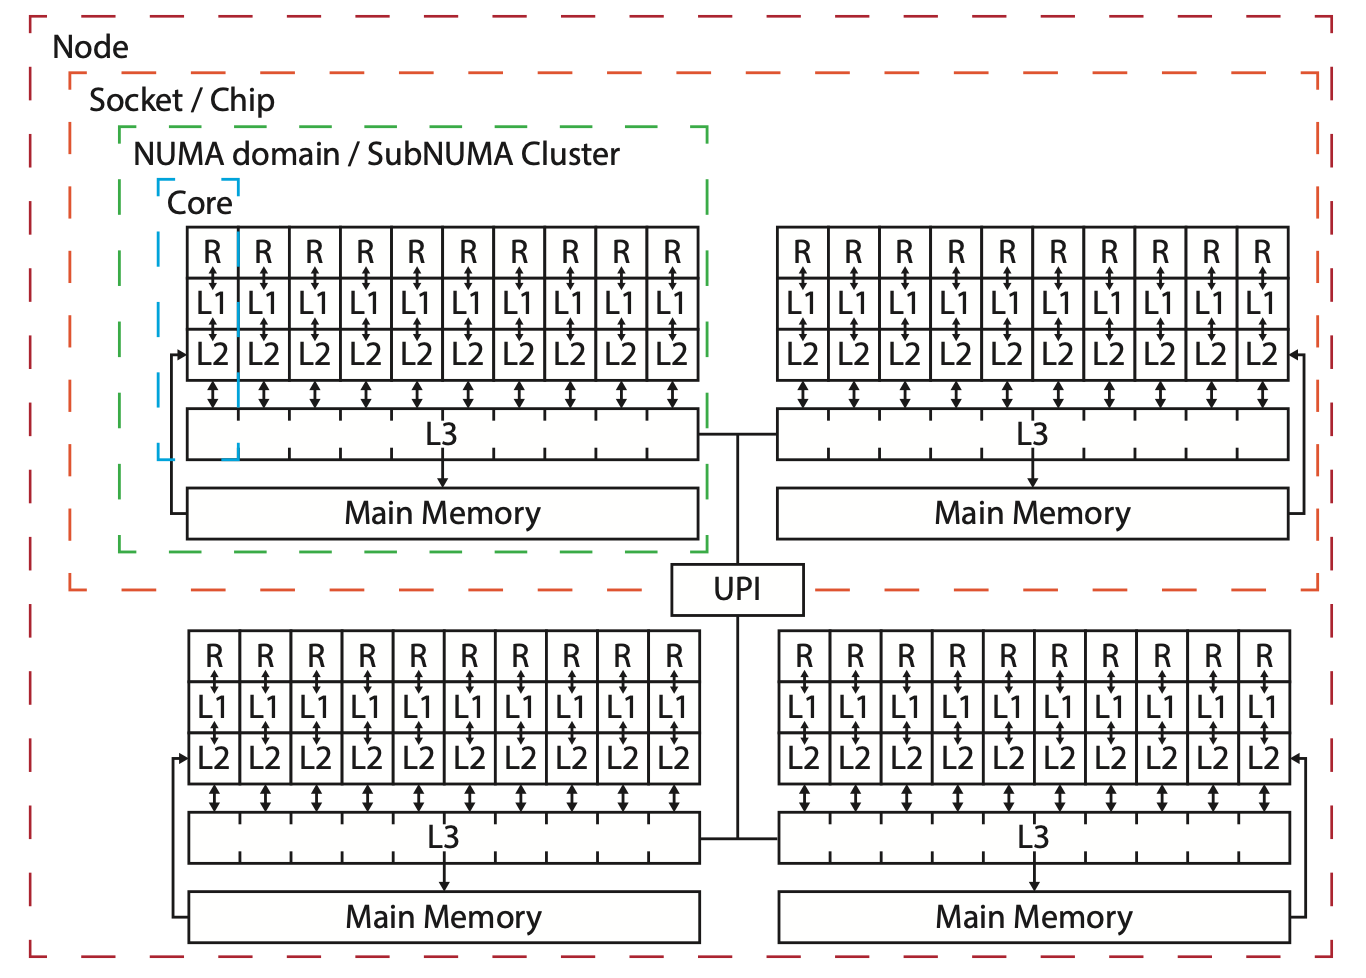
\includegraphics[width=0.75\linewidth]{img/xeon-architecture.png}
    \caption{Intel Xeon Skylake-X CPU distribution of cores and caches. Figure adapted from \autocite{phd-apmtrlk}}
    \label{fig:xeon-layour}
\end{figure}

The traditional layout of these \glspl{cpu} can be found from \autoref{fig:xeon-layour}, where each ten cores form a \gls{NUMA} domain, two \gls{NUMA} domains for each of the chips (sockets) and multiple chips (two in this case) form a \gls{NUMA} node.


\begin{figure}
    \centering
    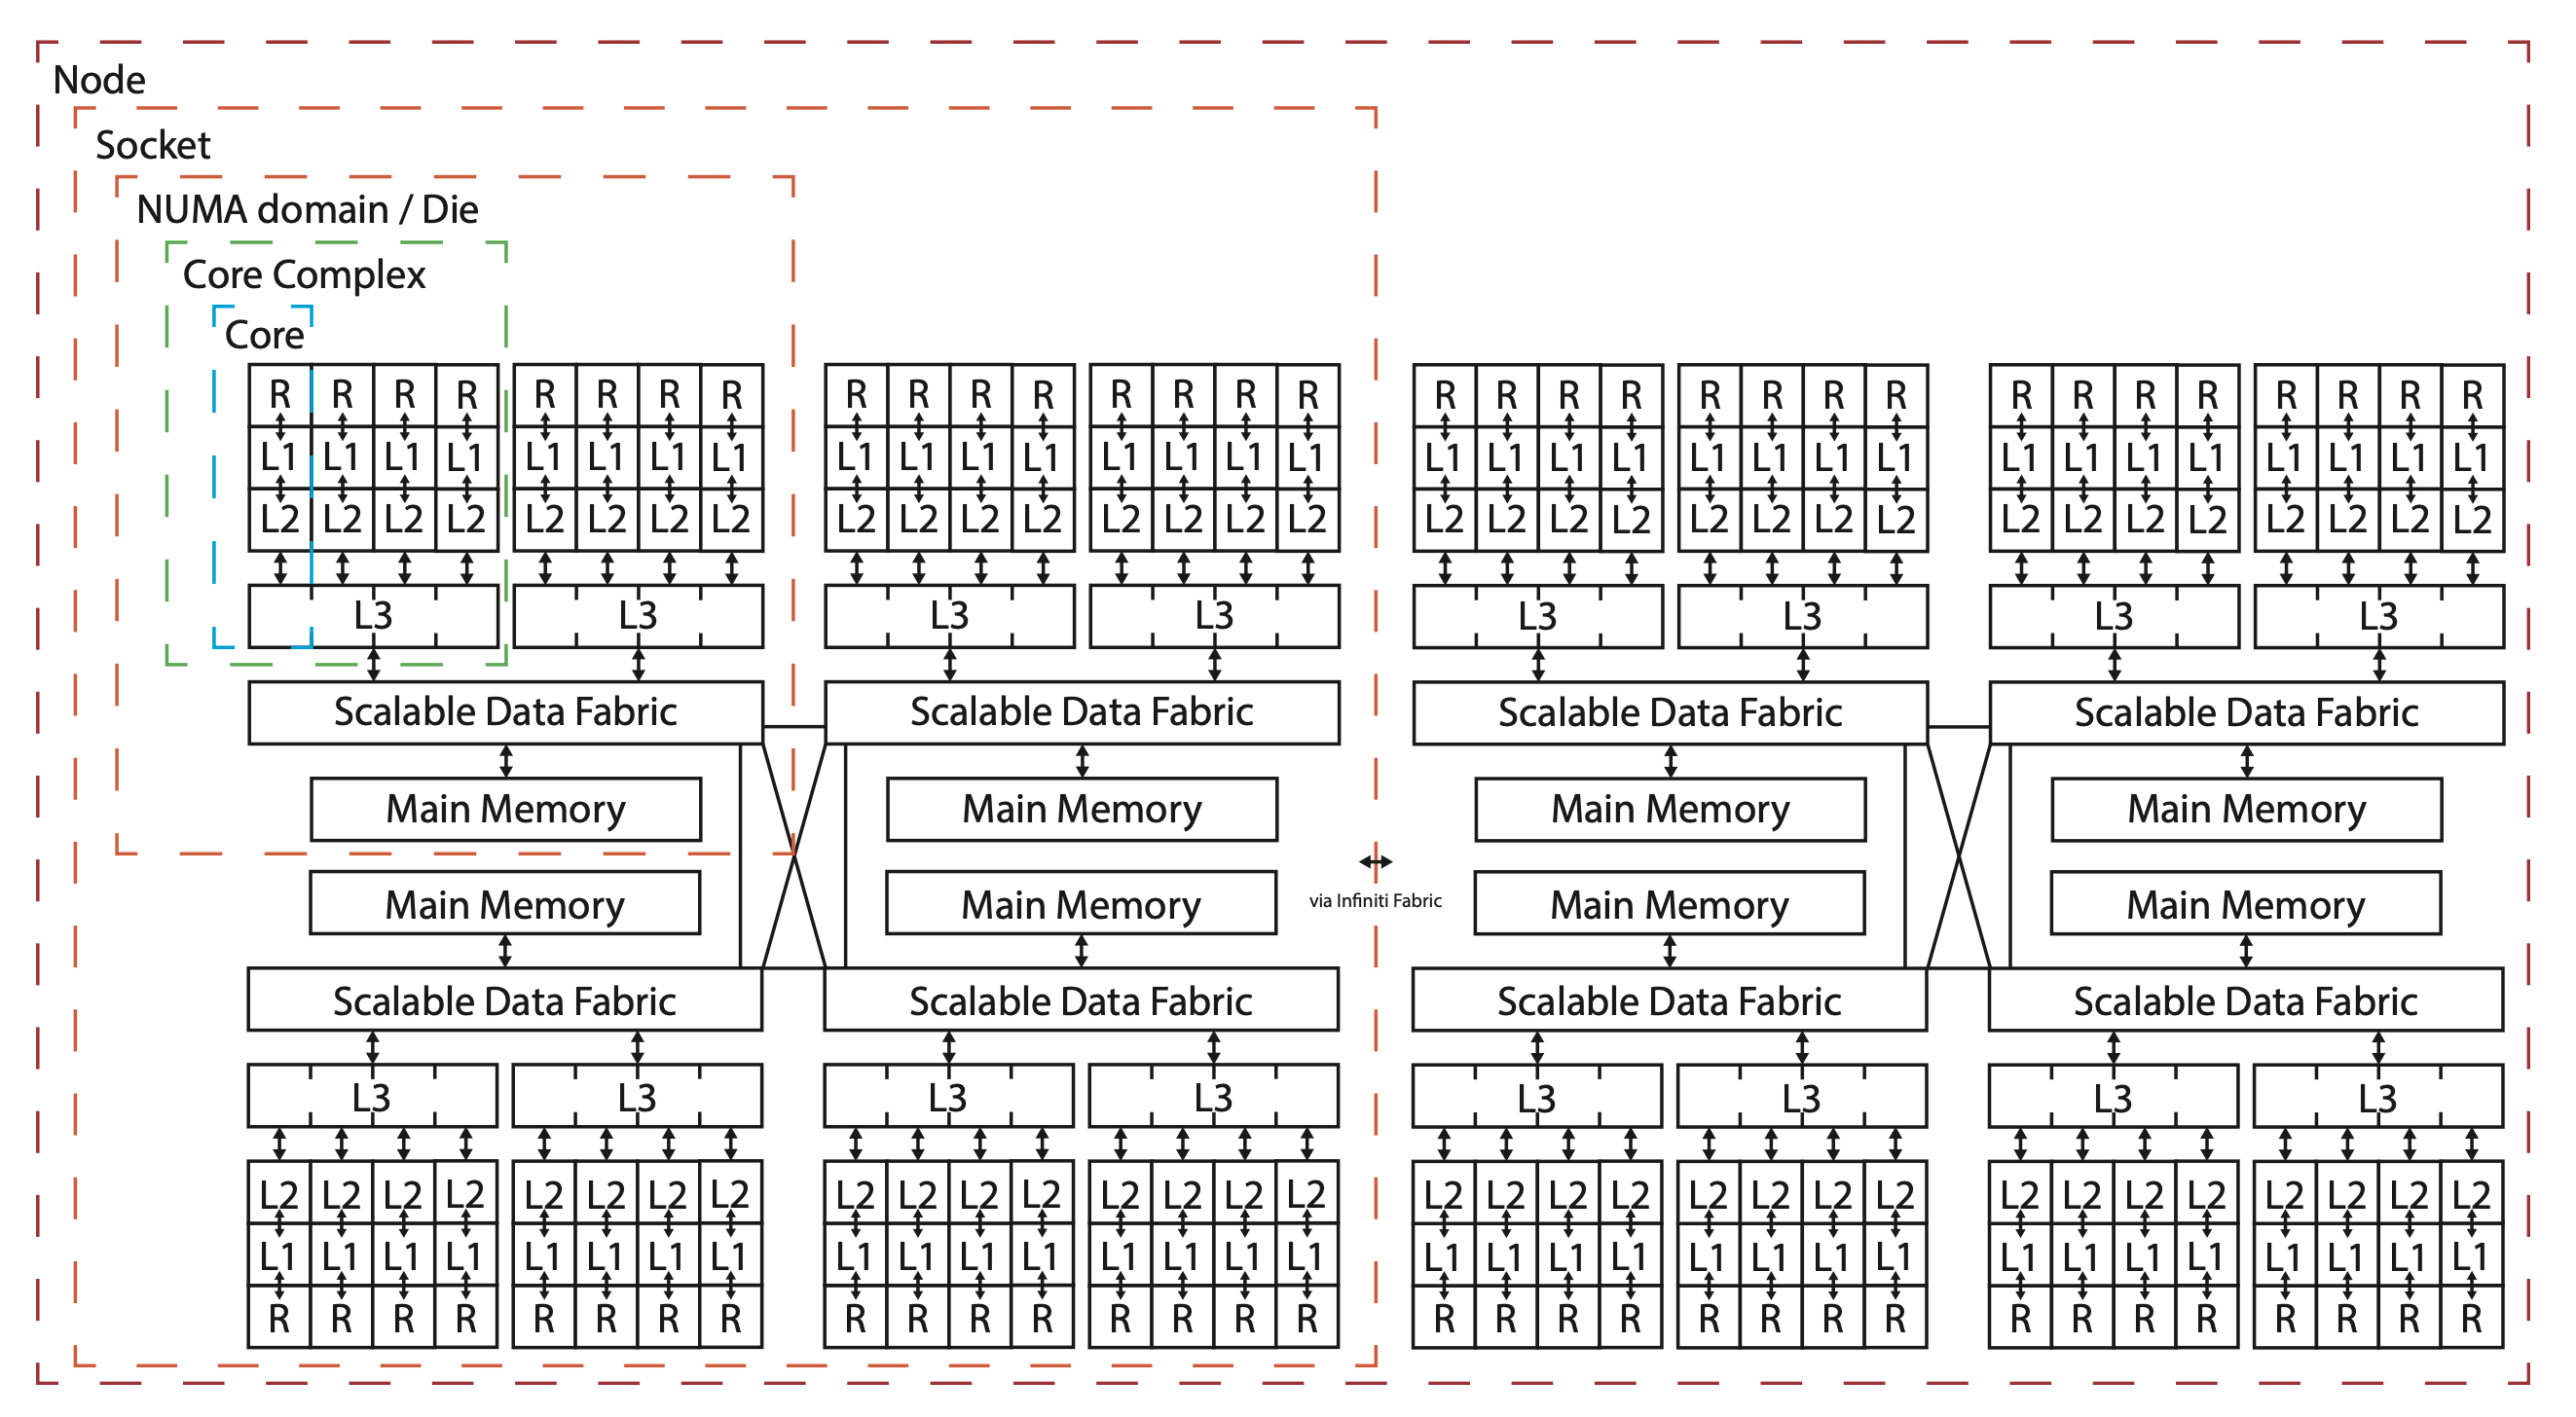
\includegraphics[width=0.85\linewidth]{img/ccx-zen2-layout.png}
    \caption{AMD's ZEN architecture. Figure adapted from \autocite{phd-apmtrlk}}
    \label{fig:zen2-architecture}
\end{figure}

AMD introduced an additional hierarchy level with its Zen architecture: \gls{CCX}. A single core complex has up to four cores, with a sliced victim L3 cache. Two \glspl{CCX} are combined onto a die, sharing a local partition of main memory. Multiple dies make up a socket, as it can be seen from \autoref{fig:zen2-architecture}.	

Using AMD's ZEN 2 architecture as a new CPU architecture example, we can observe there are is an additional layer, compared to \autoref{fig:xeon-layour}. As \textcite{zen2-architecture} puts it in their paper, in \autoref{fig:zen2-architecture}, the victim of this design is the L3 cache, which is shared between fewer cores.


\subsection{Simultaneous multithreading \& Hyperthreading}
\label{sec:hyperthreading}

SMT or Simultaneous Multithreading is a technology that allows a single physical core to appear as two logical cores to the operating system. This means that the operating system can schedule two threads on a single physical core, allowing for better utilization of the CPU resources. This usually entails a better performance, as described by \textcite{hyperthreading}.

However, for CPU-intensive benchmarks, such as floating-point operations, performance can sometimes degrade when hyperthreading is enabled. This is because the two threads share the same resources, such as the cache and execution units, which can lead to contention and reduced efficiency.

Hyperthreading is Intel's specific implmementation of SMT, which was first introduced in 2002 with the Pentium 4 processor. It has been included in most Intel processors since then, including the Core i3, i5, i7, and i9 series. AMD also has its own implementation of SMT, which is included in its Ryzen processors.

% \subsection{GPU and Accelerators}
% \label{sec:gpu-accelerators}
% The \gls{gpu} is a specialized processor designed to handle complex mathematical calculations, particularly those related to graphics rendering. It is optimized for parallel processing, allowing it to perform many calculations simultaneously. This makes it ideal for tasks such as image processing, machine learning, and scientific simulations. Most games and image renderers run using a \gls{gpu} acceleration and most AI workloads can also be accelerated by it.

% We can see from this paper \cite{gpu-energy-efficiency}, the fields where \glspl{gpu} are used are medical image processing, matrix-related computation, artificial intelligence, deep learning, etc. an acceleration of up to $50x$ can be obtained on specific kernels, compared to a \gls{cpu}.

% This would be the ideal architecture to implement our testing framework if what we were looking for is extreme performance, but, as the goal of this project is to analyze the energy efficiency of different programming languages, the \gls{gpu} is not being considered for this project. 

% An accelerator is a hardware component that enhances the performance of a system by offloading specific tasks from the CPU. Accelerators can take many forms, including \glspl{gpu}, \glspl{fpga}, and application-specific integrated circuits (ASICs). These devices are designed to perform particular computations more efficiently than a general-purpose CPU, making them valuable for tasks such as machine learning, data processing, and scientific simulations. They were very popular in the past, but their use has declined with the rise of more powerful \Glspl{cpu}.

% \subsubsection{CUDA}
% \label{sec:cuda}
% CUDA (Compute Unified Device Architecture) is a parallel computing platform and application programming interface (API) model created by NVIDIA. It allows developers to use a C-like programming language to write algorithms that can be executed on the GPU, enabling significant performance improvements for compute-intensive tasks. CUDA provides a rich set of libraries and tools for optimizing performance, making it a popular choice for high-performance computing applications. However, we will not use CUDA in this project as the focus is on analyzing the energy efficiency of programming languages rather than leveraging GPU acceleration. 
% \subsubsection{OpenCL}
% \label{sec:opencl}
% OpenCL (Open Computing Language) is an open standard for parallel programming of heterogeneous systems. It allows developers to write programs that can execute across various devices, including CPUs, GPUs, and other accelerators. OpenCL provides a C-like programming language and a set of APIs for managing parallel tasks, making it a versatile choice for high-performance computing applications. A future project could be analyzing the energy efficiency of CUDA programs vs OpenCL programs, as they are both parallel programming models for GPU acceleration.



\section{Programming Languages}

In this section, the different programming languages that have been chosen will be discussed, as well as why other similar languages were not.

\begin{table}
	\centering
	\caption{Comparison of C++, Python, and Go General Characteristics}
	\label{tab:language_comparison}
	\begin{tabularx}{\textwidth}{
		>{\raggedright\arraybackslash}p{0.18\textwidth}
		>{\raggedright\arraybackslash}X
		>{\raggedright\arraybackslash}X
		>{\raggedright\arraybackslash}X
	}
		\toprule
		\textbf{Characteristic} & \textbf{C++} & \textbf{Python} & \textbf{Go} \\
		\midrule
		
		\textbf{Typing System} &
		Statically Typed: Types are checked at compile-time, catching errors early and aiding optimization. &
		Dynamically Typed: Type checking occurs at runtime. Optional static type hinting (\href{https://peps.python.org/pep-0484/}{PEP 484}) is available. &
		Statically Typed: Types are checked at compile-time, ensuring type safety and early error detection. \\
		\addlinespace
		
		\textbf{Compilation \& Execution} &
		Compiled: Code is compiled directly to native machine code for fast execution. &
		Interpreted: Typically compiled to \gls{bytecode} which is then executed by a \gls{VM}. &
		Compiled: Code is compiled directly to a self-contained native machine code executable with a runtime. \\
		\addlinespace
		
		\textbf{Concurrency} &
		Provides primitives like threads and \gls{mutex}es, requiring manual management. &
		Offers threading (limited by the \gls{GIL} for \gls{cpu}-bound tasks) and multiprocessing libraries. &
		Built-in support with lightweight \glspl{goroutine} and \glspl{channel} managed by the Go runtime. \\
		\addlinespace
		
		\textbf{Memory Management} &
		Manual memory management, with modern C++ heavily relying on \gls{raii} and smart pointers. &
		Automatic via reference counting and a cyclic garbage collector. &
		Automatic via a concurrent, \gls{tri-color-mark-and-sweep} garbage collector. \\
		\addlinespace
		
		\textbf{Standard Library} &
		Rich library with a focus on performance (e.g., STL containers, algorithms). &
		Extensive "batteries-included" library for a vast array of tasks, speeding up development. &
		Comprehensive library designed for modern needs like networking, \gls{i-o}, and \gls{json} handling. \\
		\addlinespace
		
		\textbf{Programming Paradigms} &
		Multi-paradigm: Supports procedural, object-oriented (\gls{oop}), \gls{generic} and functional. &
		Multi-paradigm: Supports procedural, object-oriented, and functional styles. &
		Primarily procedural and concurrent. Uses composition over inheritance (no classes). \\
		\bottomrule
	\end{tabularx}
\end{table}


\begin{table} 
	\centering
	\caption{Comparison of Language Characteristics Impacting Energy Efficiency}
	\label{tab:language_comparison_energy}
	\small
	\begin{tabularx}{\textwidth}{
		>{\raggedright\arraybackslash}p{0.16\textwidth}
		>{\raggedright\arraybackslash}X
		>{\raggedright\arraybackslash}X
		>{\raggedright\arraybackslash}X
	}
		\toprule
		\multicolumn{4}{c}{\textbf{Characteristics Impacting Performance \& Energy Efficiency}} \\
		\midrule
		\textbf{Characteristic} & \textbf{C++} & \textbf{Python} & \textbf{Go} \\
		\midrule

        \textbf{Typing System} &
		Static typing and templates enable compile-time code specialization, avoiding runtime polymorphism overhead. &
		Dynamic typing limits static optimizations, as type checks and memory allocation occur at runtime. &
		Static typing allows compiler optimizations like virtualization and function inlining. \\
        \addlinespace
		
        \textbf{Execution \& Compilation} &
		Mature compilers generate highly optimized machine code, leading to shorter active \gls{cpu} time and lower energy use. &
		Code is compiled to \gls{bytecode} and run on a \gls{VM}. This interpreter overhead significantly impacts performance. &
		Compiles to efficient native machine code but needs a runtime. The compiler performs optimizations for performance. \\
        \addlinespace
        
		\textbf{Concurrency Model} &
		Low-level primitives (\texttt{std::thread}) offer fine-grained control without a \gls{GIL} but require manual management. &
		Threading is limited by the \gls{GIL} for \gls{cpu}-bound tasks. Multiprocessing works but has higher overhead. &
		Lightweight goroutines and channels allow for high concurrency with very low overhead, managed by the runtime. \\
        \addlinespace
		
		\textbf{Memory Management} &
		Manual memory control (\texttt{new}/\texttt{delete}, smart pointers) and \gls{raii} provide deterministic cleanup, avoiding \gls{GC} overhead. &
		Automatic \gls{GC} on mostly heap-allocated objects increases memory footprint, \gls{GC} load, and access latency. &
		Automatic \gls{GC} with a focus on stack allocation for value types, which reduces \gls{GC} pressure and improves data locality. \\
        \addlinespace

		\textbf{Standard Library} &
		The Standard Template Library (STL) provides highly optimized, performance-focused data structures and algorithms. &
		Performance-critical modules are often \Glspl{c-extension}, but the call overhead from Python remains. &
		Many standard library functions (e.g., networking, crypto) are highly optimized, some using assembly for critical paths. \\
        \addlinespace

		\textbf{Abstractions} &
		Aims for "zero-cost abstractions," where high-level features are compiled away and incur no runtime overhead. &
		High-level abstractions and dynamic features are powerful but generally incur significant runtime overhead. &
		Interfaces provide abstraction with a small, well-defined runtime cost. Composition is favored over inheritance. \\
		\bottomrule
	\end{tabularx}
\end{table}

\FloatBarrier

\subsection{Go: Compiled Language with an Embedded Managed Runtime}
Go is a language developed by \href{https://google.com}{Google}, released in 2009, focused on concurrency. It has a runtime which manages the \glspl{goroutine}. As described by \cite{rosecrance2019garbage}, Go has a Garbage Collector, which means while the program is running, there needs to be a thread checking for unused memory structures. 

This language was designed for backend tasks, handling thousands of simultaneous connections, while having an easy syntax for any programmer. Some companies that use this are Uber, Docker, Twitch, previously Discord \cite{discord-blog-go-rust} and, although not mainly, Netflix.

From \autoref{tab:language_comparison}, it can be seen that Go is statically typed and compiled, which makes it have a good start as an efficient programming language. But from the \autoref{tab:language_comparison_energy}, we can observe go has a managed runtime, which means the energy consumption will be higher than other languages that do not have this. This runtime is the section of the program in charge of running and scheduling \glspl{goroutine}. This is why go binaries have a bigger minimum size as the runtime has to be fitted in the binary, which is great for \gls{cross-compilation}, but not great for either energy efficiency or performance.

Go's scheduler performs a series of steps before starting to run the user's code. As described in \cite{go:GoLabConf-runtime}, \cite{go:ardanlabs-runtime} and \cite{go:memory-allocation}, the runtime can be divided into these steps:
\begin{enumerate}
    \item \textbf{OS Loading}:
    The main function is not the actual entry point of a Go program. Rather, the starting point is an assembly level function within the runtime. You can find it in a file corresponding to your specific OS and architecture, for example, \texttt{rt0\_linux\_amd64.s}. This is the first function the Go's program code will have the OS execute after loading the binary, and its only responsibility is to get the environment setup for the Go runtime.
        
    \item \textbf{Argument and Environment setup}:
        The runtime, after being loaded into memory, calls an internal function \texttt{runtime.args} that handles the arguments and environment. This function copies the arguments (\texttt{argc} and \texttt{argv}) and environment variables into a Go-managed memory space. This ensures that the rest of the Go program, including the main function, can access this information through standard library functions like \texttt{os.Args} and \texttt{os.Getenv}.
    \item \textbf{Scheduler Initialization (M:P:G Model)}:
        The heart of the concurrency system in Go is the "M:G:P" model. Before any go code is executed, the scheduler must be initialized, which happens inside \texttt{runtime.schedinit}.
        \begin{itemize}
            \item \textbf{\texttt{M0} and \texttt{G0} Creation}: The program starts with a single \gls{os} thread ($M0$). Every $M$ thread has a special \gls{goroutine} called \texttt{g0}, which is responsible for scheduling other runtime tasks.
            \item \textbf{P Initializations}: A list of \texttt{Ps} or processors, which is a resource required to execute Go code, is created. The limit of \texttt{P} is determined by the \texttt{GOMAXPROCS} environment variable or inside the  code by using the \texttt{runtime.GOMAXPROCS()} function.
        \end{itemize}
        At this time, the scheduler limits are put in place, limiting the maximum number of \gls{os} threads to 10,000.
        
    \item \textbf{Memory Allocator and \gls{GC} initialization}: Go's runtime includes a complex memory allocator and Garbage Collector \cite{go:memory-distribution} and \cite{go:memory-internals}.
    \begin{itemize}
        \item \textbf{Memory Reservation}: The runtime reserves a large region of virtual memory, divided into 3 areas: \texttt{spans}, \texttt{bitmap} and \texttt{arena} where go objects are allocated on the heap.
        \item \textbf{Allocator Structures}: Other structures such as the \texttt{mheap} (the global heap structure for Go), \texttt{mcentral} (a central cache for memory spans) and for each \texttt{P} a per-thread cache for allocating small objects without locking the main thread, called \texttt{mcache}.
        \item \textbf{\gls{GC} Pacer}: The pacer determines the optimal time to trigger a \gls{gc-cycle} based on the \texttt{GOGC} environment variable. The goal of Go's collection system is to perform one as the heap doubles in size since the previous cycle.
    \end{itemize}

    \item \textbf{Package Initialization}: At this point, the runtime can start reading from the supplied files. It starts with importing the required dependencies and initializing package-level variables. Once all files are processed in lexical file name order, the \texttt{init()} function of each file and then subsequent functions inside each file are called.

    \item \textbf{Creating the Main \Gls{goroutine}}: The runtime doesn't call the \texttt{main.main} function directly. Instead, it creates a new \gls{goroutine} to execute it. This is done using the internal \texttt{runtime.newproc} function. A new \gls{goroutine} (\texttt{G}) is created, and its instruction pointer is set to the \texttt{main.main} function. This new \gls{goroutine} is then placed into the local run queue of one of the available \texttt{P}s, making it runnable.
        
    \item \textbf{Start the Scheduler}: Finally, the \texttt{runtime.mstart} is called on the main thread, that enters into the scheduling loop. From this point on, the Go program is running, and the scheduler is fully operational, managing the execution of all goroutines on the available threads.
        
\end{enumerate}



\subsection{Python: Interpreted Programming Language}
Python is the most popular language according to the \href{https://www.tiobe.com/tiobe-index/}{TIOBE Index} as of May 2025 and has been since October 2021. Either because of its easy to start as a simple to start with programming language or because the actual trend of \gls{ai} is mostly programmed with Python, its popularity has skyrocketed.

Python, on the contrary to most of the other popular languages is an interpreted language, which means instead of having a compiler turn the code into assembly and then into binary, it has an interpreter that runs the \gls{bytecode} instructions written by the programmer one by one.

As \cite{10.1145/1103845.1094836} puts it: "Garbage collection also can have a significant impact on both execution time and memory usage, and can be fine-tuned to obtain better performance"

\subsubsection{"Compiling" Python code to \gls{bytecode}}
There are multiple steps between the Python code that the user writes and its execution. While using \gls{CPython}, the default python interpreter, this can be divided into two phases \cite{cpython-docs}:


%% -----------------
%% Pyton loop diagram with tktz
%% -----------------

\tikzset{
  block/.style = {
    rectangle,
    draw,
    fill=blue!20,
    text width=10em,
    text centered,
    rounded corners,
    minimum height=2em
  },
  io/.style = {
    trapezium,
    trapezium left angle=70,
    trapezium right angle=110,
    draw,
    fill=orange!20,
    text centered,
    minimum height=1em
  },
  line/.style = {draw, -latex'}
}

\begin{figure}
  \centering
  % Define node distance globally for the picture
  \begin{tikzpicture}[node distance = 1cm and 1.5cm]
    % Place nodes using the positioning library syntax
    \node [io] (bytecode) {Bytecode Sequence};

    \node [block, below = of bytecode] (fetch)
      {a. Fetch next bytecode instruction};

    \node [block, below = of fetch] (decode)
      {b. Determine instruction's meaning (Decode)};

    \node [block, below = of decode] (execute)
      {c. Execute the instruction};

    \node [block, below = of execute] (move)
      {d. Move to next instruction};

    \node [io, right = of execute, xshift=1.5cm, text width=5em] (data)
      {Manipulate Call Stack \& Data Heap};

    % Draw arrows (your path commands were already perfect)
    \path [line] (bytecode) -- (fetch);
    \path [line] (fetch) -- (decode);
    \path [line] (decode) -- (execute);
    \path [line] (execute) -- (move);

    % Arrow showing interaction with data/stack
    \path [draw, <->, -latex'] (execute.east) --
      node[midway, above, text width=2cm, text centered] {Read/Write}
      (data.west);

    % The loop back arrow using orthogonal paths
    \path [line] (move.west) -- ++(-1.5, 0) |- (fetch);

  \end{tikzpicture}
  \caption{Python’s Execution loop}
  \label{fig:python-loop}
\end{figure}


\begin{enumerate}
    \item \textbf{Phase 1: The "Frontend"} 
    \begin{enumerate}
        \item \textbf{Reading the source code}: The python interpreter reads the \textit{.py} files that were passed as an argument when invoked.
        \item \textbf{Lexical Analysis (Lexing \& Tokenizing)}: In this step, the interpreter breaks down the code into a sequence of tokens, the smallest meaningful unit of the language's grammar.
        \item \textbf{Parsing}: The stream of tokens from the previous step is fed into the parser, which checks if the sequence of tokens conforms to the rules that define Python's grammar \cite{python_grammar_ref}.
        \item \textbf{Compiling to \gls{bytecode}}: The \gls{AST} is traversed generating \gls{bytecode}. When the compilation is done, python caches the bytecode into a folder names \texttt{\_\_pycache\_\_} and stores \texttt{.pyc} files, representing the \gls{bytecode} version of the same named file, so that in future executions, all the previous steps can be skipped.
    \end{enumerate}
    \item \textbf{Phase 2: The "Backend"} 
    \begin{enumerate}
        \item \textbf{Loading the \gls{bytecode}} into the \gls{PVM}, either from the output of the compiler or from the \texttt{.pyc} file.
        \item \textbf{Python's Execution loop}: As we can see form \autoref{fig:python-loop}, the loop is extremely simple. It starts by fetching the next instruction, decoding that instruction, executing it and moving the pointer to the next instruction.
        \item \textbf{Stack Frame Management}: The \gls{PVM} manages function execution by pushing a stack frame, containing the function's context like its variables and return address, onto the call stack upon invocation and popping it upon completion to resume the prior state.
        \item \textbf{Memory Management}:
        \begin{itemize}
            \item Reference Counting: This is the primary mechanism. It works by having all objects keep a count of how many variables or other objects refer to themselves. If this count drops to zero, the object is removed from memory and thus that section of the memory is freed.
            \item Cyclic Garbage Collector: As there are some cases where the reference counting can not deal with cyclic references (e.g., when object $\alpha$ refers to $\beta$ and $\beta$ refers to $\alpha$), a garbage collector process also has to run periodically. This means the efficiency of the interpreter is not very high as it need extra processes to clean up memory. This \gls{GC} uses a generational approach, based on the idea that most objects are short-lived, and focuses its effort on newer objects. \footnote{In some interpreters such as \gls{CPython}, you can interact with the collector using the \textbf{gc} module. \cite{python-gc} } 
        \end{itemize}
    \end{enumerate}
\end{enumerate}

%% -----------------
%% Python dissasembly example
%% -----------------

\lstdefinestyle{pythonstyle}{
    language=Python,
    backgroundcolor=\color{black!5},   % light grey background
    commentstyle=\color{green!40!black},
    keywordstyle=\color{blue},
    stringstyle=\color{purple},
    numberstyle=\tiny\color{gray},
    basicstyle=\ttfamily\small,        % use a typewriter font
    breakatwhitespace=false,         
    breaklines=true,                 
    captionpos=b,                    % puts the caption at the bottom
    keepspaces=true,                 % respects spaces, crucial for Python
    numbers=left,                    
    numbersep=5pt,                   % space between line numbers and code
    showspaces=false,                
    showstringspaces=false,
    showtabs=false,
    frame=single,                    % adds a frame around the code
    rulecolor=\color{black},
    tabsize=2
}

% Apply this style to all listings environments globally
\lstset{style=estilo}

\section*{A Concrete Example with \texttt{dis}}

% --- PYTHON CODE LISTING ---
\begin{lstlisting}[language=Python, caption={Python code demonstrating the \texttt{dis} module.}, label={lst:dis_example}
]
import dis

def simple_math(a):
    x = a + 10
    return x

# Use the disassembler to inspect the function's bytecode
dis.dis(simple_math)
\end{lstlisting}

Let's see this in action. The \texttt{dis} module is a "disassembler" that 
shows you the bytecode for a piece of Python code. The script in \autoref{lst:dis_example} defines a simple function and then uses \texttt{dis} to inspect it.

\begin{lstlisting}[
    language={}, 
    caption={Bytecode output generated by the \texttt{dis.dis} function.},
    label={lst:dis_output}]
  4           0 LOAD_FAST                0 (a)
              2 LOAD_CONST               1 (10)
              4 BINARY_ADD
              6 STORE_FAST               1 (x)

  5           8 LOAD_FAST                1 (x)
             10 RETURN_VALUE
\end{lstlisting}

The output of this script, shown in \autoref{lst:dis_output}, reveals the  low-level bytecode instructions that the Python Virtual Machine will execute.




\subsubsection{Other Interpreters}

\begin{table}[h]
    \centering
    \caption{Alternative Python Implementations}
    \label{tab:python_implementations}
    \begin{tabular}{ll}
        \toprule
        \textbf{Implementation} & \textbf{Description} \\
        \midrule
        IronPython & Python running on .NET \\
        MicroPython & Python running on microcontrollers and in the Web browser \\
        Stackless Python & A branch of CPython supporting microthreads \\
        Jython & Python running on the Java Virtual Machine \\
        \bottomrule
    \end{tabular}
\end{table}

As python's interpreter is almost completely independent of its syntax and language development, there are multiple interpreters, each one with its features. One of the most popular alternatives to \gls{CPython} is \href{https://pypy.org/}{PyPy}, a fast implementation of Python with a \gls{jit} compiler. The problem with Just in Time compilers are that there might incur into potential warmup costs, before the functions go through the compiler. This process can optimize some hot code paths (a function or a section of the code that is run multiple times). Other examples are shown out in \autoref{tab:python_implementations}



\subsection{C++: Directly Compiled, Unmanaged Language}
Based on the programming language C (high-level language at the time, compared to assembly, in 1972), C++ was released in 1983. Nowadays, it is known as one of the most famous languages when it comes to high performance computing applications.

As we can see from \autoref{tab:language_comparison}, there are many characteristics on why it is one of the most used languages for high performance software, for example, blender\footnote{\href{https://blender.org}{blender.org}} or nuke\footnote{\href{https://www.foundry.com/products/nuke-family}{nuke.com}}. These known examples and the multiple tests performed in multiple courses during the computer science degree have shown its capabilities.


If we take into account the energy efficiency, from \autoref{tab:language_comparison_energy} we can observe that being a compiled language, with multiple optimizations at the compilation level, zero-cost abstractions and direct memory management makes it one of the best low energy consumption language in theory.
In this section, the different programming languages that have been chosen will be discussed, as well as why other similar languages were not.



\subsubsection{Compilers}

There are three main compilers for C++: \textbf{G++}, \textbf{Clang++} and \textbf{MSVC}. As this project is being done on a Linux system, I will only be using G++ and Clang++.

\textbf{G++} is the C++ compiler for the GNU Compiler Collection (GCC). It is widely considered as a seasoned, reliable veteran; it's the default on most Linux distributions and has a long history of producing highly optimized code for final release builds. While its error messages have improved significantly over the years, they can sometimes be verbose and a bit cryptic, leaving you to decipher a long template expansion error.

\textbf{Clang++} is the C++ compiler front-end for the \gls{LLVM} project. It often feels like it was designed specifically to make a developer's life easier, excelling in two key areas: speed and diagnostics. Clang++ is famous for its remarkably fast compilation times and for error messages that are not only clear and color-coded but often suggest the exact fix, creating a much tighter and less frustrating coding loop. This focus on tooling is why it's also the engine behind many modern IDE features and static analysis tools.


\subsection{Other languages not used}

There are many more languages, but to reduce the scope of the project and have a good analysis on each of the languages to be analyzed, a reduced group had to be selected. 

As a contender for a fast, high energy efficient language we could have used Rust, a recently new programming language, focused on performance and type-safety. As Rust is a compiled language and uses the same \gls{LLVM} backend for compilation, a similar result is to be expected from this benchmark compared to the C++ implementation, thus, I excluded it from the study.

Other languages that, while not necessarily the most efficient, could have been strong candidates for testing due to their widespread adoption are listed in \autoref{tab:excluded_languages}

\begin{table}
	\centering
	\caption{Languages Excluded from the Study and Justification}
	\label{tab:excluded_languages}
	\begin{tabularx}{\textwidth}{
		>{\raggedright\arraybackslash}p{0.18\textwidth}
		>{\raggedright\arraybackslash}X
	}
		\toprule
		\textbf{Language} & \textbf{Reason for Exclusion} \\
		\midrule
		
		\textbf{Java / C\#} &
		These languages primarily execute on managed runtimes (the JVM and .NET CLR, respectively). Their common Just-In-Time (JIT) compilation model is fundamentally different from the Ahead-Of-Time (AOT) native compilation of C++ and Go. Including them would be similar to go's implementation with a specific runtime . \\
		\addlinespace
		
		\textbf{JavaScript / TypeScript} &
		These languages were designed for more web-centric environments, these languages run on JavaScript engines and typically use a single-threaded event loop for concurrency. This distinct execution paradigm and primary application domain fall outside the scope of this study, which focuses on general-purpose compiled languages. Some runtimes that JavaScript use are Node, Deno or bun, but all of them have to use a core, either \gls{V8} (for node and Deno) or JavaScriptCore (for bun). \\
		\addlinespace
		
		\textbf{Ada} &
		While a statically typed and being Ahead-of-time compiled language, Ada is highly specialized for high-integrity, real-time, and safety-critical systems (e.g., avionics, defense). Its lower mainstream adoption and niche focus make it less representative for this study. \\
		\addlinespace
		
		\textbf{Zig} &
		As a modern systems' language, Zig aligns well with the technical characteristics of C++ and Go. However, it is a relatively new language that has not yet achieved the same level of industrial adoption, ecosystem maturity, or long-term stability as the selected languages. The study's focus is on established, widely-used technologies to ensure the relevance of the findings to the current software development landscape. \\
		\bottomrule
	\end{tabularx}
\end{table}


\section{Previous Benchmarks}

Research in this area has intensified recently, driven by the growing global imperative to improve energy efficiency. This topic is no longer a niche concern but has garnered significant interest across industrial, economic, and policymaking sectors worldwide.

One of the first papers published that sparked the flame in the energy efficiency aspect of software development is \textcite{energy-efficiency-rui-v1}, that analyzed the performance of twenty-seven languages in ten different programming problems. The problem I found out with these kinds of tests is that the algorithms usually are quite simple and do not represent real-world applications. 

As \textcite{vankempen2025itseasygreenenergy} put it, "Despite the fact that these studies are statistical and only establish associations, they have nonetheless been broadly interpreted as establishing a causal relationship, that the choice of programming language has a direct effect on a system’s energy consumption. This misinterpretation stems in part from the work’s presentation, not only in ranking of languages by efficiency, but also from the specific claim that “it is almost always possible to choose the best language” when considering execution time and energy consumption \cite{ranking-rui-pereira}". Continuing with that idea, they also state that short benchmarks are not realistic of a real-life program being executed on a machine.

The most important aspect of comparing two languages when doing a benchmark, is making sure that the algorithm used to solve the task is the same between the multiple languages. Thus, the benchmarks that test the languages using libraries sometimes poison the results by adding another language without their knowledge. For instance, if the python program uses \texttt{\gls{numpy}}, most of that library is implemented in C, or if we were to use \texttt{\gls{PyTorch}}, that library is mostly implemented in C++-

Other studies such as \cite{ranking-rui-pereira}, specifically on their Table 3, on the top languages, for \texttt{binary-trees}, \texttt{fannkuch-redux}, and \texttt{fasta}, are C, C++, Rust and \gls{fortran}, exchanging positions depending on the test. As we see from this list, these are all compiled languages, which is not a surprise, as \textcite{imact-compiler} comment on their paper comparing multiple compiler flags and other languages. 

As \textcite{usenix-comparing-29x} state in their publication "studies have found that \gls{V8} and \gls{CPython} can be $8.01$x and $29.50$x slower on average that their C++ counterparts respectively" but they also state that, "choosing a language for your application simple because it is 'fast' is the ultimate form of premature optimization" \cite{python-is-slow}. They have also found out that with respect to a language with a runtime, it can provide a better performance and scalability. Although this might be counter-intuitive, Go's scheduler automatically maps user threads to kernel threads thus reducing the number of context switches.

Another challenge this area faces is measuring the energy consumption. Some \glspl{cpu} have internal registers that can provide these measurements, like the intel \gls{RAPL}, but other machines might have those registers not accessible to the user or, in case of most \gls{ARM} processors, these registers do not exist. Another technique is using the measurement from an external power plug, like the TP-link HS110, used by \textcite{meassuring-jit} in their measurements. The problem with these kinds of measurement devices it that the entire system is measured instead of only the \gls{cpu} or the \gls{ram} and the precision it provides is much lower, being able to read only at a $1$ Hz frequency. 

